

\section{ScopeSim Architecture}
\label{scopesim-architecture}

In order to work as a multi-purpose optical\footnote{Optical refers to the wavelength ranges where telescopes act as ``photon buckets'' and detectors are in essence ``photon counters'', i.e.~from the near ultraviolet ($0.1\,\micron$) to the mid infrared ($30\,\micron$).} instrument simulator, \ScopeSim{} needs to be able to handle (at least) the two main types of instruments: imagers and spectrographs.

While every instrument is unique, all instruments, by virtue of their astronomical nature, have several key aspects in common.
All instruments:

\begin{itemize}
\item transport incoming photons through an optical system towards a detector (array),

\item use a limited number of optical components, e.g: mirrors, lenses, and gratings,

\item are only a single element in a combined optical train, which includes the atmosphere, telescope, and relay optics,

\item introduce a series of optical aberrations depending on the configuration of the optical system,

\item are generally built to behave in a predictable and repeatable manner.
\end{itemize}

These five points are important to recognise, as they have the following consequences:

\begin{itemize}
\item each optical element is responsible for one or more optical aberrations, which are not dependent on the aberrations inherent to the other optical elements,

\item the effect of each aberration on the spatial and spectral distribution of photons remains constant for a given optical configuration,

\item this constancy means the characteristics of these effects need only be calculated once and can be described by an analytical function, or an empirical data set,

\item common elements (e.g.~telescopes, atmospheres, etc.) of complex optical trains can be re-used with different instruments to create new combined optical systems.
\end{itemize}

This list of consequences implies that the final observed image from a telescope/instrument optical system is simply the sum of a discrete number of independent optical effects repositioning the incoming photons on the focal plane.

While this conclusion may seem obvious and trivial, by using it as the basis for \ScopeSim{}, it has allowed us to design and build a flexible, lightweight, general purpose instrument simulator that is capable of simulating the majority of current and future optical astronomical instruments.
\ScopeSim{} is able to mimic the optical aberrations seen in imagers, long-slit and multi-object spectrographs, as well as integral-field spectrographs.
The architecture could also theoretically be used to simulate high-contrast and high-time-resolution imagers, however these systems have not yet been tested.


\subsection{Simulation workflow}
\label{simulation-workflow}

The main \ScopeSim{} engine architecture is based around five major Python classes:

\begin{itemize}
\item \textbf{\Source{}}: holds a spectro-spatial description of the on-sky target.

\item \textbf{\FieldOfView{}}: extracts quasi-monochromatic flux maps from a \Source{} object and projects these into focal plane coordinates.

\item \textbf{\ImagePlane{}}: mimics the focal plane and acts like a 2D canvas for collecting the flux maps held in the \FieldOfView{} objects.

\item \textbf{\DetectorArray}: mimics the functionality of the instrument detector array in converting the final expectation flux image from the \ImagePlane{} into FITS format pixel maps similar to those delivered by the system's read-out electronics.

\item \textbf{\Effect{}}: the interface base class for introducing spectral and spatial aberrations into the final flux map.
\end{itemize}

Figure~\ref{fig:workflow} illustrates how the first four of these classes interact with each other.
The \Effect{} class is described separately in Section \ref{effects-objects}.

\begin{figure}

\resizebox{\linewidth}{!}{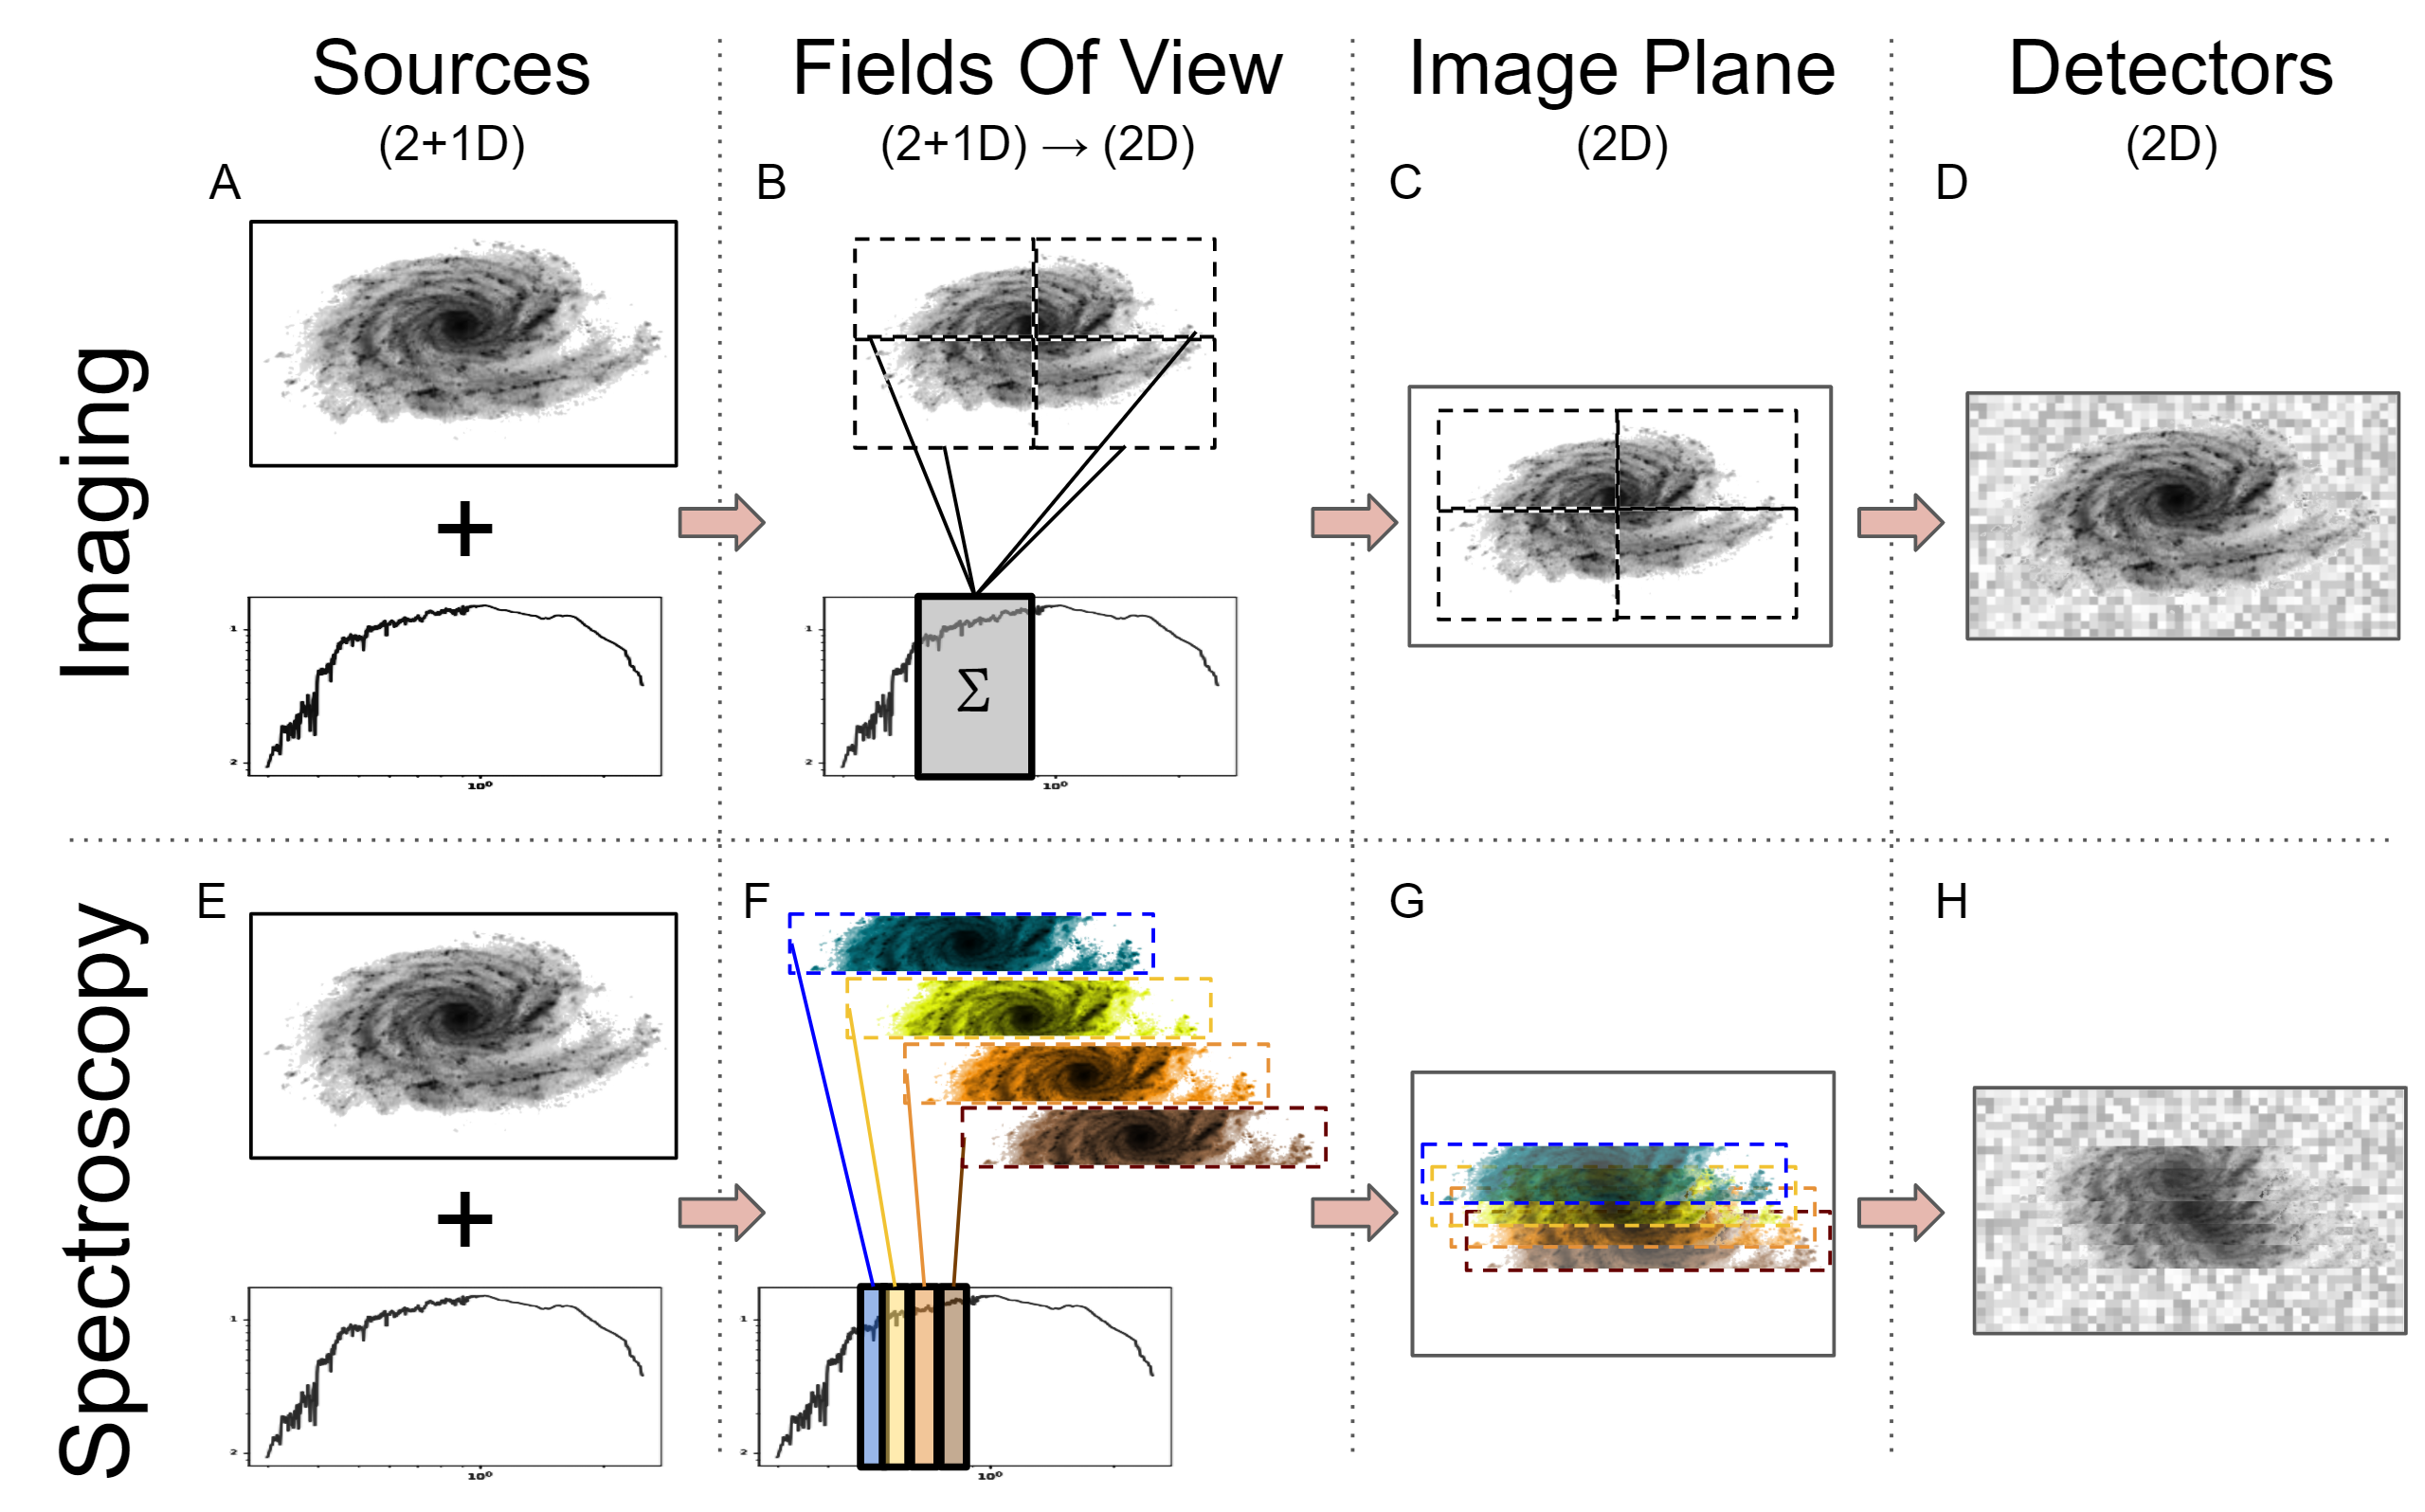
\includegraphics{Workflow.png}}
\caption{An illustration of the connections between the main internal classes in \ScopeSim{}: \Source{}, \FieldOfView{}, \ImagePlane{}, \DetectorArray{}.
The upper panels show the work flow for imaging simulations.
The lower panels show the work flow for spectroscopy simulations.
The work flow is in principle the same for both types of simulation.
(A, E)~Both modes require a 2+1D description of the on-sky target(s) containing linked spatial~(2D) and spectral~(1D) information.
The main difference lies in how and where the spatial and spectral borders for each \FieldOfView{} object are set.
\FieldOfView{} objects~(B, E) extract (2D)~integrated photon maps from the \Source{} object(s) and project these onto an \ImagePlane{} object.
This creates a normalised expectation image, similar to what happens at the detector focal plane in a real instrument.
The \DetectorArray{}~(D, H) extracts the regions of the \ImagePlane{} that each detector chip would see.
Simulation output in both imaging and spectroscopic cases is the same: A FITS file with detector read images in the same format as generated by the real instrument.}
\label{fig:workflow}

\end{figure}

The \Source{} objects~(A, E) are supplied by the user.
These contain a 2+1D description of the on-sky target(s).
The spatial (2D) information is stored either as tables (collection of point sources) or as \lstinline{ImageHDU} objects (for extended objects).
Each of the spatial ``fields'' must be accompanied by one or more unique spectrum.
There need not be a one-to-one relationship between the spatial and spectral inputs.
Multiple spatial fields can reference a single spectrum.
In doing so, \ScopeSim{} can vastly reduce the amount of data that needs to be processed.
For example, a star cluster will contain many thousands of point sources.
However, only several tens of spectra are needed to adequately describe all the stars in the cluster.
There will be many hundreds of M-type stars that can reference a single common M-type stellar spectrum.

\ScopeSim{} builds a model of the optical train by importing instrument packages.
Based on the list of \Effect{}s contained in the configuration files, \ScopeSim{} splits the full spectral and spatial parameter space of the instrument into 3D ``puzzle'' pieces, known as \FieldOfView{} objects.
Each \FieldOfView{} object~(B, F) then extracts only the flux from the \Source{} object that fits within its spectro-spatial limits.
This process essentially creates a series of quasi-monochromatic puzzle pieces from the 2+1D source flux.
The spatial size and spectral depth of each puzzle piece is determined by which optical effects are included in the optical model.
For imager instruments where chromatic effects rarely play a large role, the spectral depth of each \FieldOfView{} object will be relatively large.
It is not uncommon for the spectral depth to be equal to the width of the filter bandpass.
The on-sky area for an imager is generally very large and so the viewing area is split into multiple pieces.
This is illustrated in the upper half of panel~B in Figure~\ref{fig:workflow}.
For spectrographs, the spatial component is generally small (e.g.~long slits, MOS fibre heads).
The spectral space however must be very finely sampled to accurately reproduce the spectral traces on the focal plane.
Spectrographic optical systems therefore contain many \FieldOfView{} objects which cover the same on-sky spatial region, yet cover very shallow and unique spectral ranges.
The \FieldOfView{} objects also contain two sets of spatial coordinates which connect the object's position on sky (in units of arcseconds from the optical axis) to the projected position on the detector focal plane (in units of millimeters from the optical axis).

The \ImagePlane{}~(C, G) inside each optical model acts as a 2D canvas for the integrated flux contained inside the \FieldOfView{} objects.
When each \FieldOfView{} object deposits its flux map onto the \ImagePlane{}, it simply adds the photon counts to what is already on the canvas at the \FieldOfView{}'s projected focal plane position.
The resulting \ImagePlane{} image is therefore the final integrated projected expectation flux map as would exist at the detector focal plane of a real image, in units of $\mathrm{ph\,s^{-1}\,pixel^{-1}}$.
All information on telescope aperture, viewing angle, and spectral bandpass has been integrated into the normalised photon count map -- thus the name ``expectation'' flux map.
At this stage of the simulation all sources of background flux (atmospheric, thermal) have also been projected onto the \ImagePlane{}, but no noise characteristics are included.

The \DetectorArray{} class contains a list of \Detector{} objects (D, H).
\Detector{} objects extract a region of the \ImagePlane{}'s expection flux map corresponding to its own footprint on the detector focal plane and scales this to match the user's desired exposure time (DIT in seconds).
The resulting image is the flux that a real detector would register in an ideal world.
At this point all noise characteristics are introduced, e.g.~shot noise, read noise, dark current, etc.
The final detector output is returned in the form of a FITS \lstinline{HDUList} object.


\subsection{Effect Objects}
\label{effects-objects}

\begin{figure}

\resizebox{\linewidth}{!}{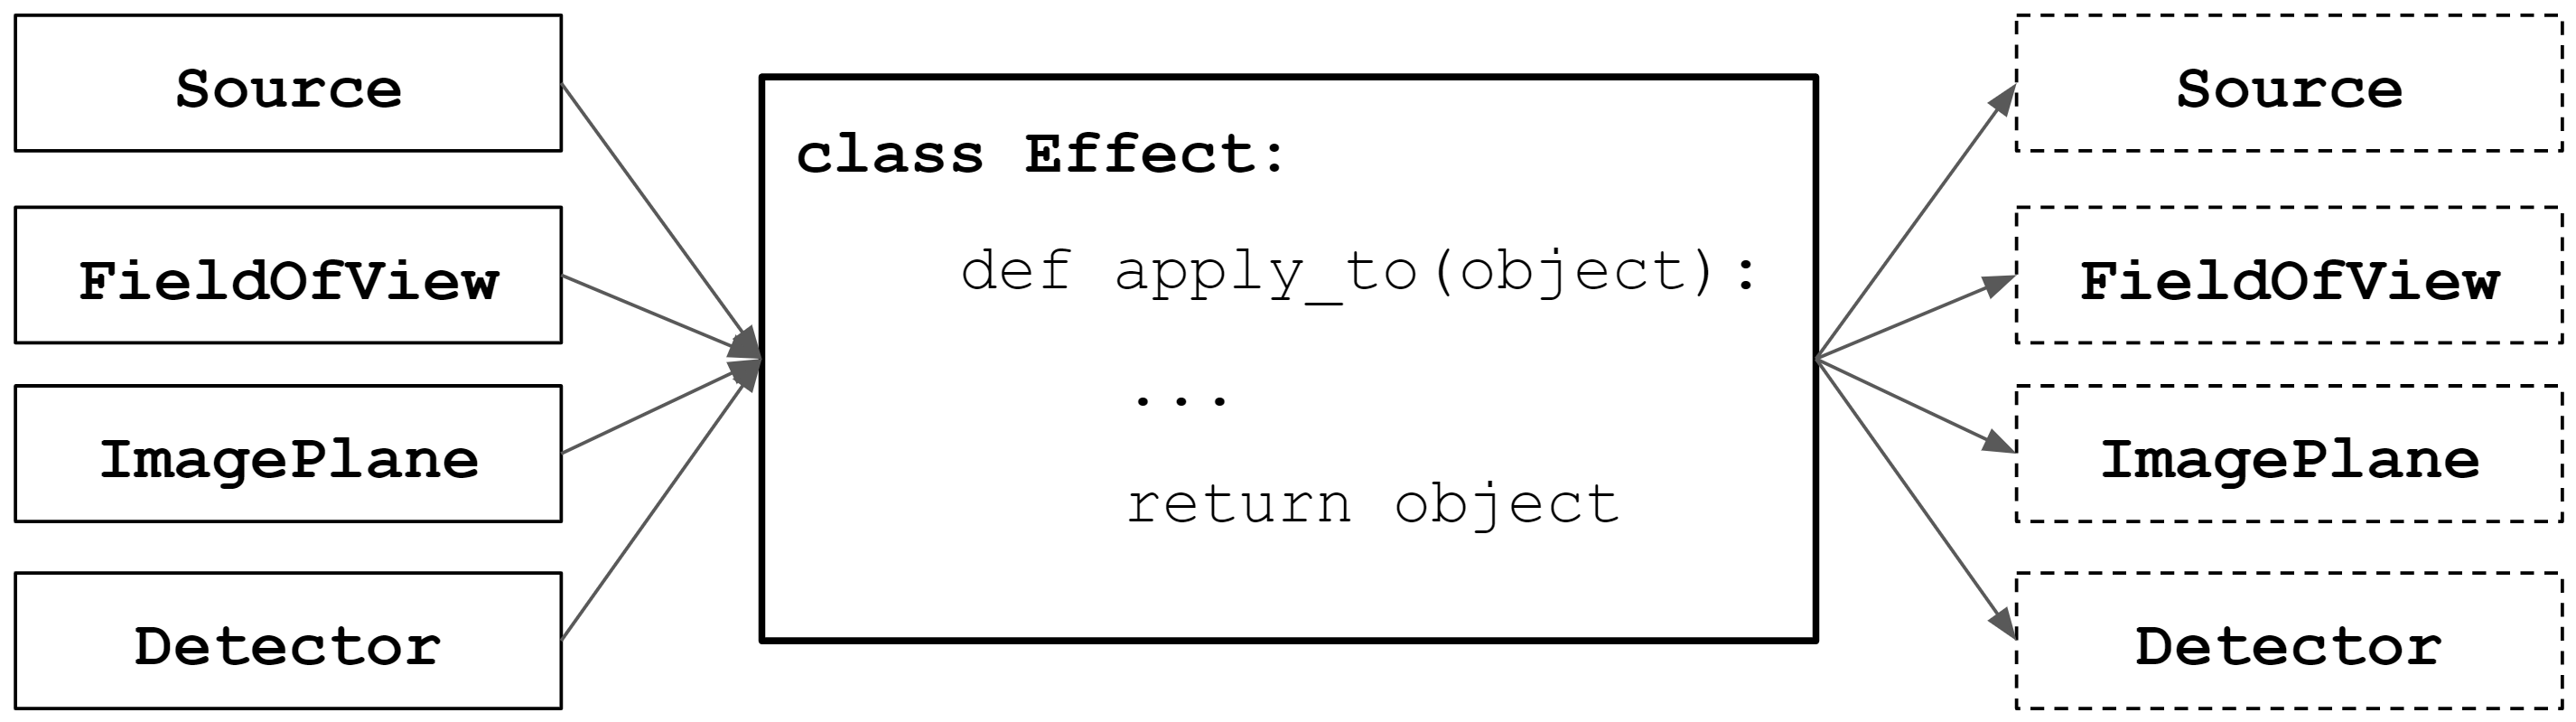
\includegraphics{Effects.png}}
\caption{\Effect{} objects modify the contents of their input objects but preserve their class.
%Effect objects are similar to mathematical operators.
%What goes in must come out.
Each \Effect{} object has a single point of entry: the \lstinline{apply_to} method, which can accept any one of the four major \ScopeSim{} classes.
This method is responsible for applying optical aberrations to the flux distribution contained within those four major flux container classes.}
\label{fig:effect}

\end{figure}

A further special (and arguably the most important) \ScopeSim{} class is the \Effect{} object.
\Effect{} objects are responsible for applying any and all optical aberrations to the flux descriptions contained in the other four major flux container classes.
\Effect{} objects can contain code to alter the flux descriptions in a multitude of manners, from simple 0D alterations like adding a dark current to each pixel, to the 3D chromatic shear caused by atmospheric refraction.
In short, \Effect{} objects can be classified according to the dimensionality of their alterations to the flux descriptions:

\begin{itemize}
\item 3D: Effects are spatially and spectrally dependent aberrations, e.g: the broadband point spread function, atmospheric diffraction, etc.,

\item 2D: Effects are only spatially dependent, e.g: telescope vibration and wind shake, pupil tracking rotations, etc.,

\item 1D: Effects are only spectrally dependent, e.g: reflection and transmission curves, quantum efficiency, etc.,

\item 0D: Effects are spectrally and spatially independent. This are primarily effects that are related to photons counts and electronic noise sources, e.g:
Poisson shot noise, read-out noise, exposure stacking, detector linearity, etc.
\end{itemize}

Higher dimensional Effects are also possible albeit very rare, e.g. field varying PSFs.

Functionally, the \Effect{} class is an ``endomorphic'' operator class.
This dictates that an \Effect{} object may alter the contents of an input object, but it must not alter the input object's class type.
In other words, if a \Source{} object is the input to an \Effect{} object's \lstinline{apply_to} function, then a \Source{} object will also be returned.
%The \Effect{} object may alter the distribution of flux inside an object, but it must return the same object.
This is illustrated in Figure~\ref{fig:effect}.

During the simulation workflow, the target object flux makes its way through the four main class objects described in Section~\ref{simulation-workflow}.
While flux resides in each of these objects, the relevant \Effect{}s are sequentially applied to said object.
For example, the telescope's (chromatic) PSF is applied to each of the \FieldOfView{} objects, as this is a spectrally dependent spatial (3D) effect.
In contrast, the wind-shake gaussian PSF has no spectral dependency and is therefore only applied to the \ImagePlane{}.

The following pseudo-code snippet describes the major steps of the simulation workflow and illustrates how and when the Effect objects interact with the four major flux container classes:

%\begin{quote}
%\begin{alltt}
%\begin{minipage}[c]{0.95\textwidth}
\begin{lstlisting}[frame=single]
source = deepcopy(orig_source)

for effect in source_effects:
    source = effect.apply_to(source)

fov.extract_from(source)

for effect in fov_effects:
    fov = effect.apply_to(fov)

image_plane.add(fov)

for effect image_plane_effects:
    image_plane = effect.apply_to(image_plane)

detector.extract_from(image_plane)

for effect detector_effects:
    detector = effect.apply_to(detector)

detector.write_to("file.fits")
\end{lstlisting}
%end{minipage}
%\end{alltt}
%\end{quote}

As can be seen, there is a very similar pattern.
Obviously there are a few more steps involved in the actual \ScopeSim{} code, however the \lstinline{observe} method of an optical model consists of little more than a Python implementation of this pseudo-code.

\ScopeSim{} already includes a large number of standard \Effect{}s in the core package, including, but not limited to: PSFs, transmission curves, Filter wheels, atmospheric dispersion, detector readout noise models, etc (see online documentation for a full list).
It is clear however that there are many more that could be added.
The \Effect{} object interface has been intentionally kept light weight to encourage users to implement custom effects for their own simulations.
The online documentation contains a tutorial on how to write custom effects.
Users are also cordially invited to submit any custom \Effect{}s they deem useful to the wider community to the \ScopeSim{} package as a pull request via the Github repository.
